%!TeX program=pdflatex
%!TeX encoding=utf8
%!TeX spellcheck = en_US
%!TeX root = ../../messageVortex.tex

\part{Results\label{sec:results}}
To verify the hypothesis made in this paper and to analyze the properties of the protocol in a real-world scenario, we implemented a library in Java. This library is capable of handling all message packets and the routing stack as a whole. The implementation is available under \url{https://messagevortex.net}. The following paragraphs describe the protocol developed in general as a generic approach. Appendix \ref{app:rfcMessageVortexMain} gives the full ASN.1 representation of the protocol. 

As ASN.1 has no means to express encrypted structures, we defined all encrypted fields as \verb|OCTET STRING|. The protocol supports onionized information in an unencrypted form. These unencrypted structures are for debugging purposes only. At no point should this possibility be used in a production environment.

The protocol described in the next chapter is independent of routing. We built a blending layer for SMTP. Layers for other protocols such as XMPP may be defined similarly. We extend the protocol by adding new blending layers for the transport protocol and their addressing schemes.

The Protocol outlined here is the final product and has undergone many development cycles. We dropped a lot of advantageous features and capabilities, such as a mechanism analogous to the SMTP received headers, as they were beneficial but threatened security or anonymity.

\chapter{Vortex Prerequisites}
\section{Hardware}
We require no specialized hardware for running Vortex nodes. Instead, we designed Vortex in such a way that ordinary mobile phones may act as Vortex nodes. It is, however, recommended to have a node always connected to the Internet. A mobile phone may disconnect from time to time based on the availability of the network. For our experiments, we used a RaspberryPi Zero W. It is, however, recommended to use a faster, newer model due to the memory requirements of the proof of work algorithm. 

The hardware currently requires a network interface and a fully functional JSE VM to run the reference implementation.

\section{Addresses}

A Vortex address is built as follows: 

\begin{lstlisting}[language=EBNF]
localPart         = <local part of address>
domain            = <domain part of address>
email             = localPart "@" domain
keySpec           = <BASE64 encoded AsymmetricKey [DER encoded]>
smtpAlternateSpec = localPart ".." keySpec ".." domain "@localhost"
smtpUrl           = "vortexsmtp://" smtpAlternateSpec
\end{lstlisting}

To allow storage of Vortex addresses in standard messaging programs such as Outlook or Thunderbird, we introduced $smtpAlternateSpec$. 

The suffix ``@localhost'' makes sure that any non-participating server does not route a message intended for Vortex. The doubly dotted notation is not RFC compliant but was accepted by all tested client address books. The address is, however, not a valid SMTP address due to its double-dotted notation. We selected this representatiopn to differentiate Vortex addresses from valid email addresses.

The main downside of vortex addresses is that they are no longer readable by a human. The main reason for this is the public key, which is required. We may abstract this further by allowing clear-text requests on the primary email address for the public key. The vortex account must then answer such requests with the valid Vortex address.

The $smtpUrl$ is representing the address in a standard way, which makes it suitable for QR codes and intent filters on Android.

The public key of an address is encoded as follows:
\begin{enumerate}
	\item The asymmetric key is encoded as specified in the AsymmetricKey in ASN.1
	\item The ASN.1 DER representation is then encoded using BASE64
\end{enumerate}    

\section{Transport Layers}                                          
As transport layer protocols, we specified the protocols SMTP and XMMP as valid transport layers. In the following sections, we specify the blending properties for these protocols.

\subsection{Embedding Spec}
We always embed VortexMessages as attachments in SMTP and XMPP messages. 

The embedding supports some properties. A receiving host chooses the supported properties. We describe valid properties by the blending specification::
\begin{lstlisting}[language=EBNF]
plainEncoding = "("plain:"<#BytesOfOffset>[,<#BytesOfOffset>]*")
F5Encoding    = "(F5:"<passwordString>[,<PasswordString>]*")"
\end{lstlisting}

We use mainly plain embedding for our experiments. For better readability, we used a specialized blending layer using unchunked, plain embedding with an offset of $0$. The message itself was the ASN.1 block representation of the encoded block. The chosen encoding simplified to see the inner workings of the protocol. For production use, we apply F5 embedding with a generated payload. The current implementation of the blending layer is thus not suitable for production use as the messages remain identifiable or at least suspicious.

\section{Client}
We did not create a Vortex client for sending messages. Instead, we used a standard Thunderbird email client pointing to a local SMTP and IMAP Server provided by a Vortex proxy. On the SMTP side, Vortex does encapsulate where possible mails into a Vortex message and builds an automated route to the recipient. The SMTP part of Vortex may be used to encapsulate all messages automatically with a known Vortex identity into a \emph{VortexMessage}. On the IMAP side, it merges a local Vortex message store with the standard Email repository building a combined view.

Using Vortex like this offers us the advantages of a known client with the anonymity Vortex offers.

Using a proxy has certain downsides. At the moment, the vortex client has only a local store. Such a local store makes it impossible to handle multiple simultaneously connected clients to use Vortex. This limitation is, however, just a lack of the current implementation and not of the protocol itself. We may safely use IMAP storage for storing \emph{VortexMessages} centrally. This statement is true as long as:
\begin{itemize}
	\item The storage is not identifiable as such.\\
	This requires:
	\begin{itemize}
		\item A non-identifiable folder/message structure
		\item A storage not identifiable by access patterns
		\item The stored messages do have the same strength as the transmitted messages in terms of detectability
	\end{itemize}
	\item A secured key\\
	Either the host key is secured sufficiently with KDF, and a passphrase (or similar), or the host key remains off-storage.
\end{itemize}

\subsection{Vortex Accounts}
By definition, any transport layer address may represent a Vortex identity. This fact may make people believe that their current email or jabber address is suitable as a Vortex address. This statement is technically perfectly true, but should not be done for the following reasons:
\begin{itemize}
	\item If an address is identified as a Vortex address, it may be blocked (directly or indirectly) by an adversary. Such blocking would lead to blocking of regular email traffic as well.
	\item If a vortex node is malfunctioning non-\emph{VortexMessages} should remain unaffected. Isolation is far better if we keep non-Vortex messages in a separate account.
	\item If a user wants no longer to maintain its Vortex address, he may give up his Vortex transport accounts. If he had been using his normal messaging account for Vortex, he would receive mixing messages which are hard to filter even with a known host key.
\end{itemize}

\subsection{Vortex Node Types}

\subsubsection{Public Vortex Node}
Public nodes are nodes, which advertise themselves as normal mixes. Just as all nodes, they may be an endpoint or a mix. Typically they accept all requests exactly as outlined in \ref{tab:protoReplyCrit}. As an immediate result of the publicly available information about such a node, the owner may be the target of our censoring adversary. Pressure may be opposed to close down such a node. However, since we do not need a specific account, we may safely close down one transport account and open up a different one. Such account reopenings are even possible on the same infrastructure. We are even able to notify other users of the move and remain reachable, as a user may send a newIdentity request using the old identity. 

\subsubsection{Stealth Vortex Node\label{sec:stealthNode}}
This node does not answer any clear-text requests. As an immediate result, the node is only usable by other nodes knowing the public key of this node. The node is, therefore, on a known secret base only reachable. This node type may be used in environments with a censoring adversary. People may form closed routing groups routing and anonymizing themselves. We have to state clearly at this point that putting trust into the routing nodes violates the \defref{Zero Trust} principle. It is, however, currently the only way to outcurve a censoring adversary. Means such as using distribution lists as endpoints seemed to be of some value at first but turned out just to shift the problem of detection from the routing to the less protected transport layer.

\subsubsection{Hidden Vortex Node\label{sec:hiddenNode}}
A hidden node is a special form to a stealth node. It has a predefined set of identities. Only these already known identities are processed. This behavior has certain drawbacks. An existing identity may not be changed, and new ephemeral identities may not be created. As an immediate result, traffic may become pseudonymity. To counter this effect, at least partially, we may use the same local identity for multiple senders. To remove clashes in the workspace, we may use preassigned IDs in the workspace. The sender is only one of all senders knowing the private key of an identity. The advantage of such a node is that identities have unlimited quotas on such nodes, no longer bothering about accounting and refreshing identities. Such behavior seems to be a valuable option when using bulletproof providers.

\chapter{Vortex Protocol Overview}
The Protocol details are described in the RFC document in \ref{app:rfcMessageVortexMain}. The RFC draft contains all the necessary information to build the protocol. The RFC is published through the official IETF channels. Besides the RFC document, additional documents and references may be found on the official website \url{https://messagevortex.net/}.

The MessageVortex protocol described here is a protocol for asynchronous data transfer. The protocol itself is embedded into a carrier protocol as binary information to avoid easy detection and make it hard to block traffic without blocking other legitimate traffic.

The data transferred is passed through multiple routers. The builder of a routing block (normally the sender) decides upon the following attributes:
\begin{itemize}
	\item Hops for the message and all decoy traffic.
	\item Timing behavior of the message.
	\item Decoy traffic generation.
	\item Set of possible recipients.
	\item Set of all nodes involved in routing.
\end{itemize}

These decisions are compiled into a routing block structure, which is onionized. This routing block may then be used to transfer a message of almost any size. This message is then sent to the involved mixes.

A mix may be just an intermediate station or the final target of a message. Only the recipient of a message can tell whether a message was intended for him or not. Any mix does a certain number of operations on a message. Considering the message, the timing and the operations applied a mix may extract the following pieces of information:
\begin{itemize}
	\item IP of the sending mix.
	\item Size of the message received.
	\item Size of all processed sub-blocks.
	\item Arrival time of a message.
	\item Ephemeral identity a message belongs to (an ephemeral pseudonym to the routing block builder (\defref{RBB})).
	\item Validity time of the message on the node.
	\item Operations applied to the message.
	\item Size of all blocks sent.
	\item IPs of the receiving mixes.
\end{itemize}

%%%%%%%%%%%%%%%%%%%%%%%%%%%%%%%%%%%%%%%%
%%% Pre-placed float
%%%%%%%%%%%%%%%%%%%%%%%%%%%%%%%%%%%%%%%%
\begin{figure*}[ht]
	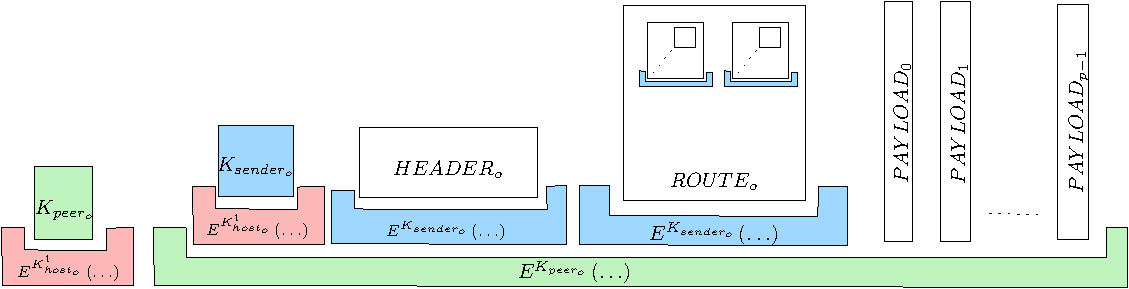
\includegraphics[width=\textwidth]{inc/blockLayoutSimplified}
	\caption{Simplified message outline}
	\label{fig:messageOutline}
\end{figure*}

A routing node always applies the operations requested in the building instructions to the received data. If this is not done, the message properly may fail to transfer to its final destination. 

The operations to be applied to a message are chosen in such a way that they may or may not generate decoy traffic. This design guarantees that valid messages or decoys may not be identified on the operations applied to the message.

Redundancy may be built in a routing block as well as progress indication.

In the taxonomy of \cite{Shirazi2018}, this protocol would be classified as follows:
\begin{itemize}
	\item Network topology: full
	\item Network connection direction: unidirectional
	\item Network connection synchronization: asynchronous
	\item Network symmetry roles: hybrid
	\item Network symmetry topology: flat
	\item Network symmetry decentralization: fully decentralized
	\item Routing network view: partial
	\item Routing updating: Event-based
	\item Communication routing type: source routed\footnote{Only partially correct, as the \defref{RBB} decides on the route. This builder is not necessarily identical to the sender.}
	\item Communication scheduling: fair
	\item Communication node selection determinism: probabilistic
	\item Communication node selection set: user-based
	\item Communication node selection probability: uniform
	\item Performance latency: high
	\item Performance communication mode: message-based
	\item Performance implementation: yes
	\item Performances code availability: yes
	\item Performance context: email, messaging
\end{itemize}

\section{Vortex Message}
The outline in figure \ref{fig:messageOutline} is a simplified view of the message block of MessageVortex.

A Vortex message is a message passed from one router to another. This message may or may not contain any valuable information. The \emph{VortexMessage} is encoded as binary data in the transfer protocol. Every router may decide for himself on the support of algorithms and embedding mechanisms.

The block structure of a Vortex message is as follows:
\begin{itemize}
	\item Encrypted peer key.\\
	It contains a symmetrical key for decryption of follow up header information and payload blocks. All symmetric keys are encrypted with a receiving host's public key.
	\item Inner Message Block (encrypted with peer key)
	\begin{itemize}
		\item header (encrypted with sender key)
		\begin{itemize}
			\item Identity 
			\item ``proof of work'' information
			\item (optionally) header requests
		\end{itemize}
		\item Routing blocks (encrypted with sender key)
		\begin{itemize}
			\item Next hop timing instructions
			\item Next hop routing blocks (encrypted)
			\item Next hop header
			\item Message build instructions.
			\item Next hop header key and spec.
			\item Next hop blending instructions.
		\end{itemize}
		\item Payload blocks
	\end{itemize}
\end{itemize}

It is important to note that there are two symmetrical keys involved in encrypting and decrypting message headers. Having two keys is not a flaw in the protocol but necessary. 

The first key of a \emph{VortexMessage} is the message key. This key is only accessible with the private key of the node receiving the message. It allows the decryption of the routing blocks and the header information. The sender of a message block is, therefore, not able to tell if a message contains one or more routing blocks. It is important to note that no other node should have access to this information. 

The second key is the sender key located before the encrypted header. The RBB chooses the key. This key protects the inner structure of the Message. It makes it impossible for any node except the sending party or the receiving peer node to detect the inner structure of the message. Without this key, any independent observer with knowledge about the blending capabilities of a receiving node may:
\begin{itemize}
	\item Easier to identify the block structure.\\ 
	This statement remains regardless of whether ASN.1 or length prefixed structures are used. If the structure of a \emph{VortexMessage} can be easily identified, the messages may be logged or dropped.
	\item Identify the routing block size.\\
	The value of this information is only minimal as it only reflects the complexity of the remaining routing information indirectly.
	\item Identify the number of payload blocks and their respective sizes. \\
	Sizing information is valuable when following the path of a message.
\end{itemize}

For the exact usage of the keys, see section~\ref{sec:keyUsage}.

It is important to note that there is no structure dividing the encrypted peer key from the Inner message block. The size of the peer key block is defined by the key and algorithm of the host key. 

\subsection{Key Usage\label{sec:keyUsage}}
Several keys are being used during the life of a message. In the following section, we emphasize on the type, the usage, and their specialties.

\subsubsection{Peer key}
The peer key is a message specific symmetrical key known to two adjacent routing nodes. It is generated by the sending routing node and encrypted with the public key of the receiving nodes identity key.

\subsubsection{Header Key}
The header key is a symmetric key protecting the routing and ephemeral identity information of the message. It is prepended to the header section and protected by the identity key of the processing node.

\subsubsection{Host Key}
The host key is a static, asymmetric keypair existing on a per-user base used to sign messages or encrypt symmetric keys. We refer here as a user any peer participating in the message stream. Every user participating in the Vortex network requires at least one key pair. 

Depending on the use-case (e.g., unlikable signatures or scalable security), a user may use multiple key pairs at the same time.

The host key is required for decrypting peer ($K_{peer}$) and sender ($K_{sender}$) key.

\subsubsection{Ephemeral Identity Key}
An \defref{eID} key identifies the sender to a processing host. The ephemeral identity key must be handled in such a way that it is not linkable. It is mainly used to process accounting information.

A user may have multiple key pairs on one routing host.

\subsection{\texorpdfstring{\emph{VortexMessage}}{VortexMessage} Processing}
A node requires FP arithmetic to process messages. To make sure that all implementations on all platforms behave the same, we always use arithmetic as specified in \citetitle{IEEE754}\cite{IEEE754}.

\subsubsection{Receiving Messages}
All messages are processed as follows:
\begin{enumerate}
	\item Extract peer key from the block. A node aborts the operation if a block is invalid or not decryptable.
	\item Decrypt sender key with hosts private key.
	\item Decrypt header block with the decrypted sender key. Abort if not decryptable or invalid block.
	\begin{itemize}
		\item Verify identity
		\item Check quotas (if any)
		\item Extract header key
		\item Extract requests (if any)
		\item Check replays (if any)
	\end{itemize}
	\item Decide if the message should be processed. If not abort here.
	\item Decrypt rest of the inner message block with the peer key
	\item Extract payload chunks.
	\item Decrypt routing blocks with header key.
	\item Check $forwardSecrets$ and discard if the inner message block contains any non-matching values.
	\item Process instructions 
\end{enumerate}

We may split the processing in an authenticated and unauthenticated processing, as shown in figure~\ref{fig:msgRecvProcessing}. When applying this 

\begin{figure*}[!ht]
	\centering
	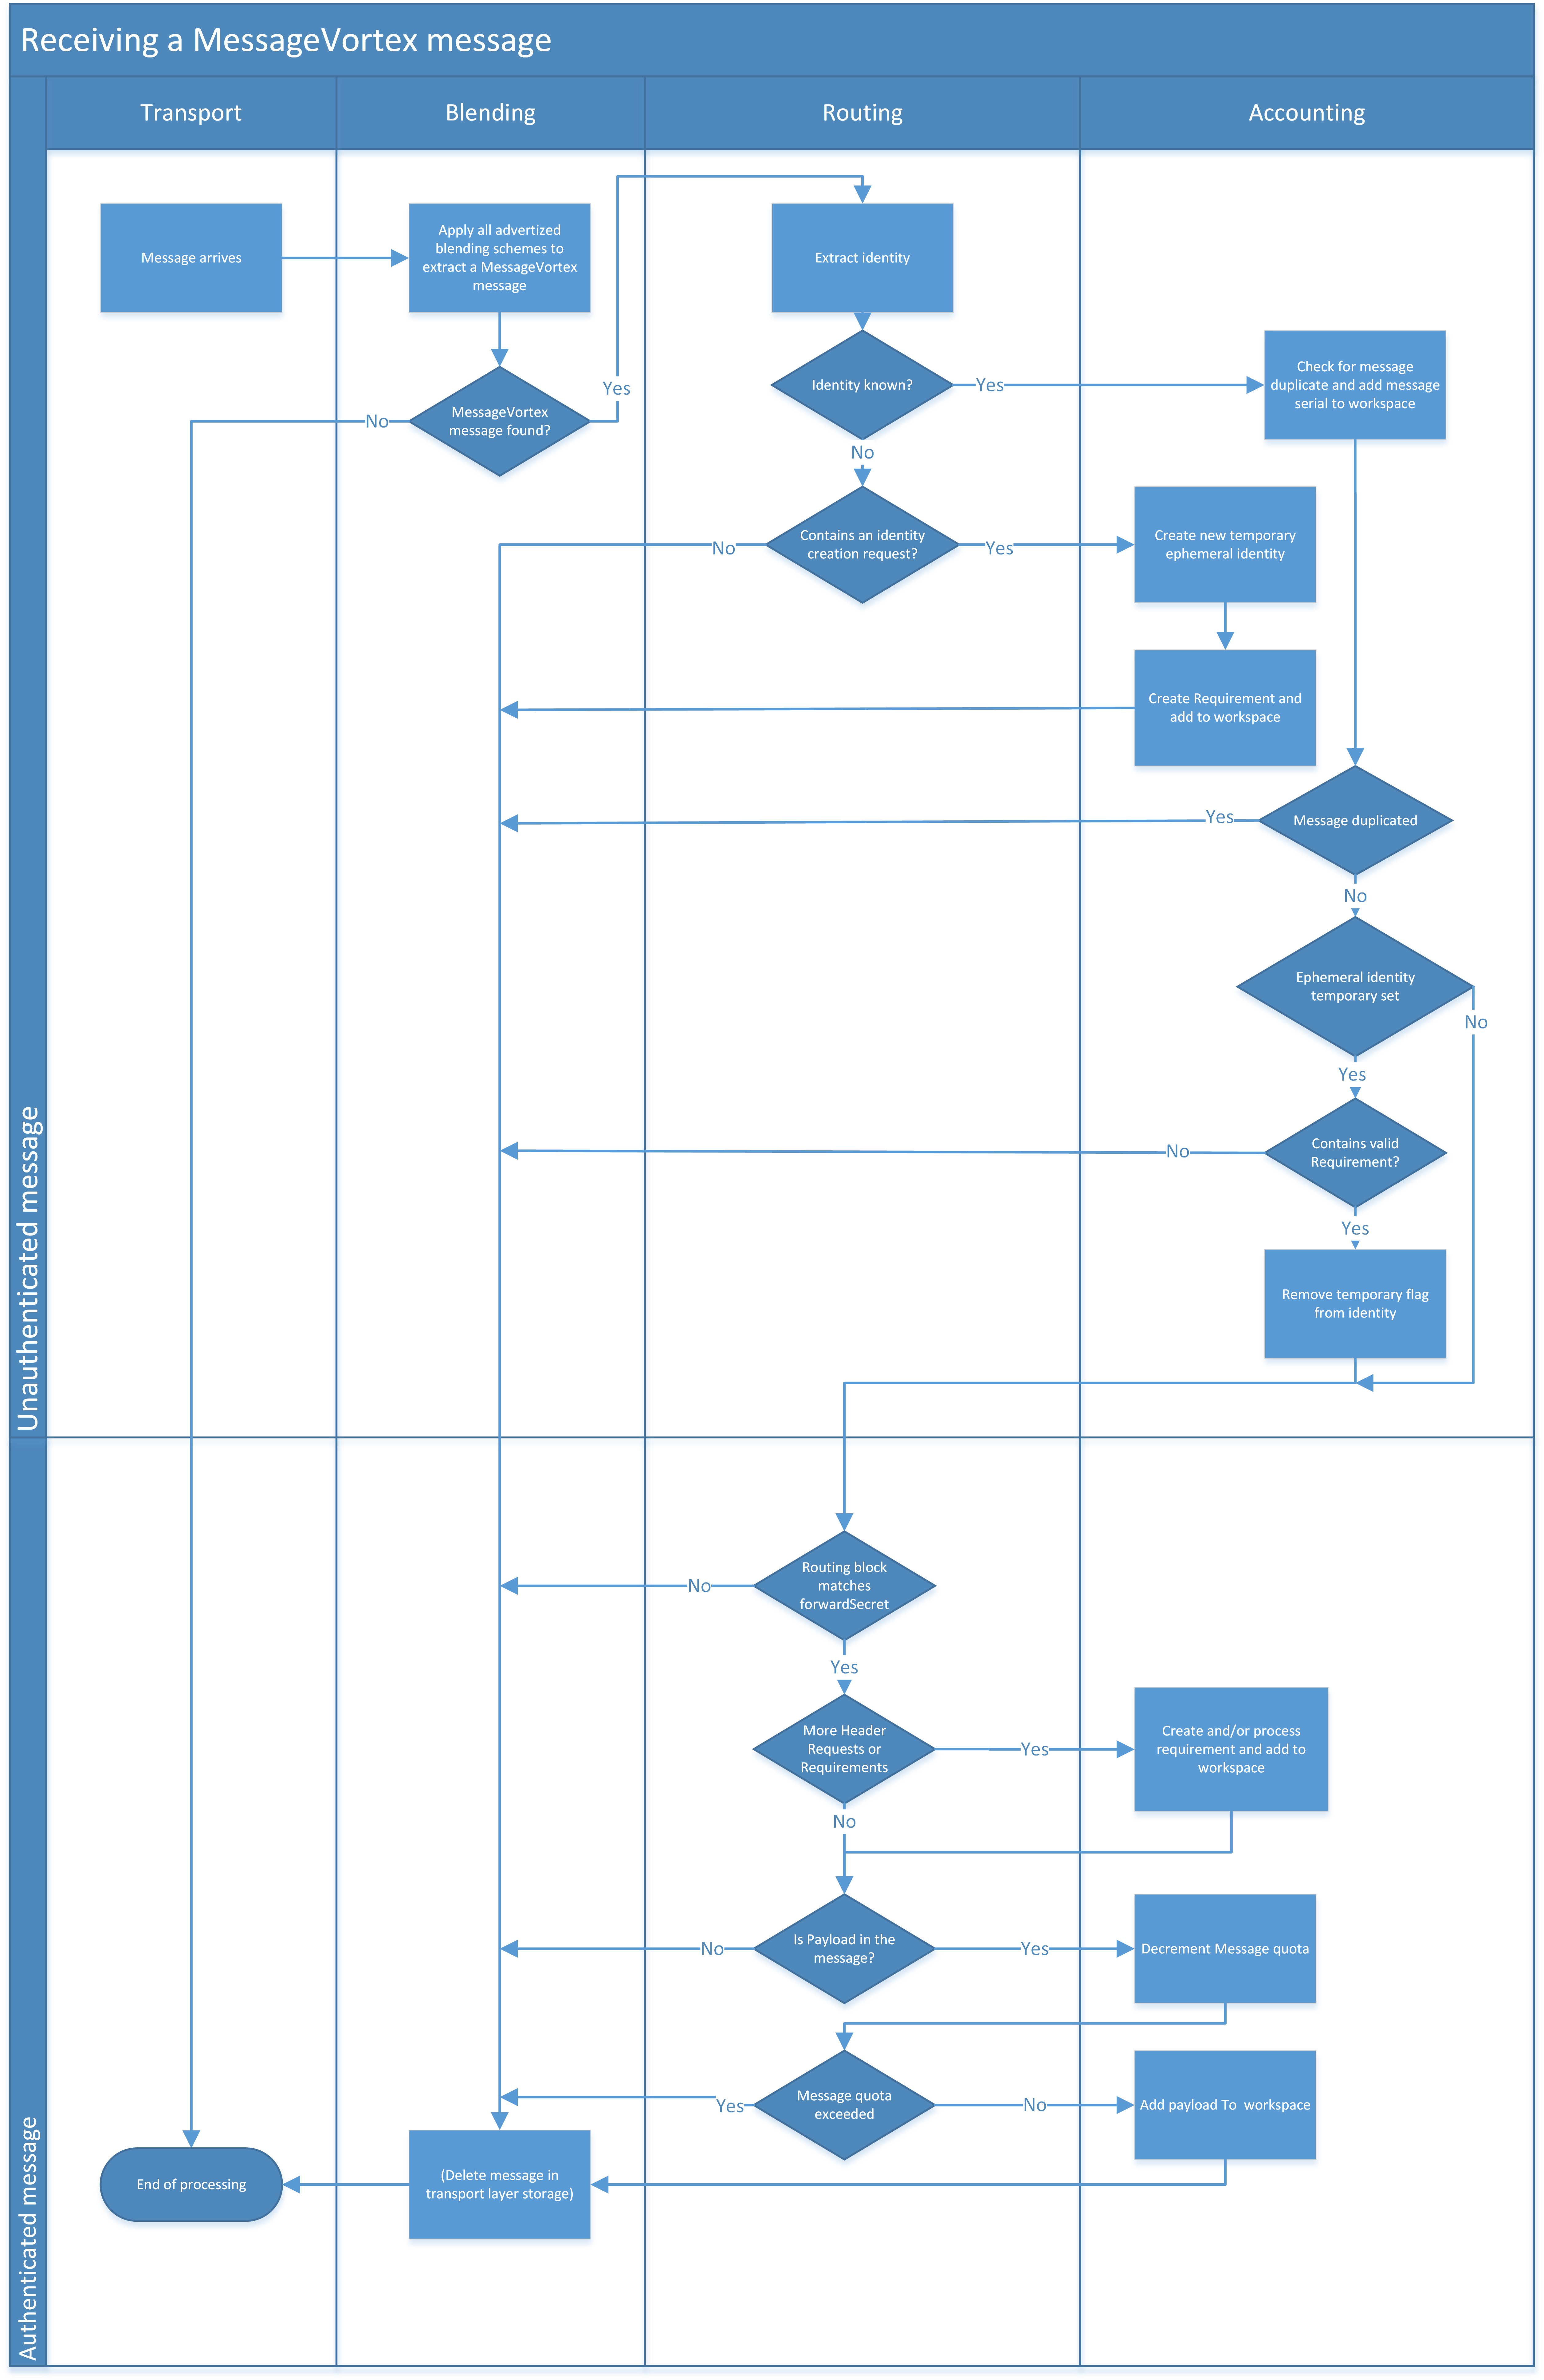
\includegraphics[width=0.80\textwidth]{inc/flowchart_message_receiving}
	\caption{flow diagram showing processing of incomming messages}
	\label{fig:msgRecvProcessing}
\end{figure*}

Every routing block creates a new message.

The payload of a message is generated according to instructions in the routing block. Timing instructions are relative to the arrival time of the message containing the routing block. This relative timing is necessary as a routing block may be used multiple times (see section~\ref{sec:murb}).

A \emph{VortexMessage} may be composed not earlier than a ``validFrom'' expressed in the respective routing block.

\subsubsection{Building and Sending Messages}
Any time after a routing block reaches ``validFrom'' and before the ``validTo'' is reached, processing of a routing block is triggered. An implementation should, when triggering a routing block for processing, trigger as many routing blocks as possible to make traffic analysis harder.

The message is then built as follows:
\begin{enumerate}
	\item Check if all building instructions can be fulfilled due to their prerequisites.
	\item Build requested payload blocks.
	\item Extract peer key from the routing block.
	\item Extract headerBlock and encrypted sender key from the routing block.
	\item Extract (sender key encrypted) nextHop routing blocks from routing block.
	\item Encrypt message using the peer key.
	\item Update accounting figures.
	\item Blend into the transport layer according to spec and send a message.
\end{enumerate}

\section{Protocol design}
In this section, we emphasize on the protocol blocks. These blocks are extracted from the blending layer and passed to the routing layer. A \emph{VortexMessage} is split into two main parts. The peer key block and the inner message block. The peer key block contains the named key in encrypted form. the inner message block contains the subparts ``senderKey'', ``header block'', ``routing block'', and ``payloads''. Although these blocks are described in \ref{app:rfcMessageVortexMain} as ASN.1 encoded structures, they are not. In the message, they are just subsequent blocks without any structure.

The reason for not using ASN.1 encoding is that it might be possible to identify the unencrypted message on the transport layer as Vortex message due to the ASN.1 structure. By not using this any supporting structure, we make it impossible for an adversary to identify the encrypted structures of a \emph{VortexMessage}.

Without the host key, it is impossible to find any structure within the encrypted message. However, assuming an existing host key detection is easy. The first block must result in an ASN.1 encoded structure containing the symmetric key (and its spec). So for detection of a message with the host key, only the decryption of a single asymmetrically encrypted block is required. A routing node uses the obtained peer key to decrypt the sender key block and the header block. After verification of the header blocks signature, a \emph{VortexNode} has all information required whether full processing is allowed or not. If so, the processing node does decrypt the routing block and check all $forwardSecrets$. After passing this test, all structures are added to the workspace of the \defref{eID}.

\subsection{Header block}
The header block contains the identity and all information required to decide whether subsequent blocks of the message should be handled.

The header block contains the following data:
\begin{itemize}
	\item An identity block (identityBlock)\\
	This block contains data reflecting the identity of the sender and the use of the header and subsequent blocks. This data includes:
	\begin{itemize}
		\item sending ephemeral identity public key (identityKey)
		\item serial number
		\item maximum number of replays for the serial for this identity
		\item Minimum number of seconds for replay protection.
		\item validity period for this block (in seconds)
		\item Chain secret for the block ($forwardSecret$)
		\item Protocol requests to this node
		\item Identifier and padding for proof of work
	\end{itemize}
	\item An identity signature (identitySignature)\\
	Contains a signed hash with the senders private key.
\end{itemize}

The identity in header blocks is always an ephemeral identity (\defref{eID}). It exists for a limited amount of time (a low number of days). Creating a new \defref{eID} is done with an identity request. 

The \defref{eID} identifies the workspace and limits the available routing capabilities. A vortex node only processes known \defref{eID}s with sufficient quotas.

\subsubsection{Requests\label{sec:request}}
Requests are always embedded in a header block. All requests are answered with a provided \defref{SURB}.

There are several header requests defined:
\begin{itemize}
	\item newIdentity request:\\
	This request may be answered with either a reject or a puzzle that is required to solve. Solving the puzzle results in the creation of the identity on the node. The node may reject identities for various reasons:
	
	\begin{itemize}
		\item The node is not accepting newIdentity requests
		\item The identity is already taken.
		\item The identity is not strong enough (it must apply stronger cryptography).
		\item The used encryption scheme is not supported by the node.
	\end{itemize}
	
	An identity may be rejected if the wrong types of keys and key sizes are used. However, it must accept at least the key types and sizes it uses for its own identity.
	
	If an identity is rejected, the request may not be replayed by the same identity again. A sending party must generate a new identity for a new request. 
	
	This request should be by far the most expensive request. It must, at any time, be more expensive to request a new identity compared to raise the quota of an existing one.
	
	An identity on this level is always ephemeral and expires after a given period. An \defref{eID} can not be prolonged for security reasons. Being unable to prolonge the lifetime of a \defref{eID} has certain drawbacks when using reply blocks. A reply block can only be valid as long as all included identities are valid. To counter this weakness without weakening security, a ctxlessNewIdentity block may be sent to a reply block owner providing him with a new reply block.
	
	\item  queryPeer request:\\
	A peer request is a request for publicly known Vortex nodes. This request does offer the possibility of harvesting the Vortex network. We hardened our system, therefore, with the following limitations to make harvesting harder:
	\begin{itemize}
		\item The request is very costly
		\item Only nodes advertising themselves as ``public'' are disclosed.
		\item Only one or two nodes should be disclosed upon request.
		\item A node should always pick random nodes out of a 5\% pool of known Vortex addresses.
	\end{itemize}
	
	These measures limit the effectivity of harvesting attacks while giving any node the possibility of bootstrapping itself.
	
	
	\item $queryCapabillity$ request:\\
	This request is the only request answered as a clear-text request. We minimize the possibility of probing by answering such requests only if the node owner agrees to it or generally by public nodes.
	
	\item $messageQuota$ request:\\ 
	This request raises the number of routing blocks which may be processed for an identity. A node may reject this request depending on the load of the node, personal preferences, or because this identity causes too much traffic.
	
	It is typically answered for all valid identities only. The node should reject even recently \defref{eID}s. A routing node should, however, not send a reply to an unknown \defref{eID} as this behavior might be used for the probing of a node.
	
	\item $transferQuota$ request:\\
	This request raises the number of bytes that may be transferred for an identity. A node may reject this request depending on the current load, personal preferences, or because this identity causes too much traffic.
	
	The same restrictions as in $messageQuota$ apply.
	
	\item $queryQuota$ request:\\
	This request instructs the node to send information about the given identity.
\end{itemize}

It is typically answered for all valid identities only. The node may have recently expired. It is, however, not recommended to send a reply to an unknown identity as this behavior might be used for the probing of a node.

\subsubsection{Replys to Clear Text Requests}
It is up to the decision of the node whether it wants to answer a clear-text request or not. Recommended for this behavior is to discard plain text requests. 

Discarding such requests should only be a problem when bootstrapping or when adding new identities to their address book. 

\subsection{Routing Blocks}
Routing blocks contain an onionised route, chosen by the builder of the routing blocks, and may provide instructions for building subsequent messages.

Routing blocks contain the following information:
\begin{itemize}
	\item The node specification of the next hop (requires a full identity; may be missing  if there is no next hop)
	\item The moment of processing as a range in seconds since the time of arrival.
	\item Retention time in seconds since the time of arrival.
	\item The key blocks for the next hop
	\item The peer key in plain
	\item The identity block for the next hop
	\item The routing block for the next hop
	\item Payload building instructions
\end{itemize}

\subsubsection{Payload Building Instructions\label{sec:buildInstr}}
Payload is being built right before sending a block (processing a routing block). The building instructions are built as follows:
\begin{equation*}
srcIDs \xrightarrow{\text{build operation}} targetIDs
\end{equation*}

Every node maintains a list of received blocks, including their IDs and building instructions for them. Any node must keep blocks and building instructions during the whole lifetime of a routing block. It may keep it longer. If a conflicting building instruction arrives, all conflicting older rules are removed. Building instructions are always referring to the workspace of the signing \defref{eID}. It is not possible to reference building instructions of a different identity.

\begin{itemize}
	\item splitPayload and mergePayload: \\
	Split a message block into two parts of varying sizes. The size of the first chunk is expressed either absolute or in percent of the original block size.
	\item encryptPayload and decryptPayload:\\ 
	Encrypts and decrypts a payload chunk block with a given symmetric key and algorithm. Please note that this operation changes the size of a message due to the key size and the padding.
	\item addRedundancy and removeRedundancy:\\
	Splits a payload block into uniform chunks and adds redundancy information or removes it.
\end{itemize}

All the operations specified above have in common that they may be applied to decoy traffic as well as on real message data. The size of incoming and outgoing blocks do not relate as messages are increasing the size as well as decreasing in size.

We describe the operations in detail in section~\ref{sec:operations}.

\subsubsection{payload Block}
The payload block contains the actual message or decoy traffic. Since this block is heavily modified in the course of the transport of the block, it is built simplistically. It contains only the payload data. 

An active adversary may always replace a payload block when routing. Any tagging introduced by an active adversary at this point does invalidate the stream. The output after the next hop is entirely unpredictable and, thus, tagging ineffective.

\subsubsection{Reply Block\label{sec:replyBlock}}
Reply blocks are blocks embedded into payload blocks. There are very few reply blocks necessary. Unlike normal data blocks, these messages are not accounted to quotas on the node generating the reply block. 

It is up to the node to decide whether it wants to answer a request or not.

Replies are being built as ordinary message blocks. To identify a Vortex message, it must begin with the string ``\textbackslash special'' encoded in ASCII followed by a valid reply block structure. No additional bytes may be appended. Blocks with other data should be discarded. To express a block starting with ``\textbackslash special'', the token is repeated prefixed with a backslash.

\begin{itemize}
	\item $replyCapability$ block:\\
	The reply contains the following information:
	\begin{itemize}
		\item Supported Vortex transports, including blending specification.
		\item Maximum quota.
		\item Supported ciphers and hashes.
		\item Maximum number of simultaneous valid header serials.
		\item Maximum number of simultaneous valid building operations.
		\item Maximum identity lifespan in seconds.
	\end{itemize}
	It lists the capabilities a node advertises to the public. 
	
	\item $requirement$ block:\\
	Requirement blocks denote a requirement a requester has to fulfill before a previously sent request is processed. Usually, proof of work puzzles needs to be solved to allow a request to be processed. Alternatively, a commercial supplier may request payment in digital currency. Currently, supported digital currencies are Bitcoin, Ethereum, and ZCash.
	
	\item $replyStatus$ block:\\
	General answer block, which is signaling a status. The block is limited in length to minimize the misuse of bandwidth. The Block contains the following data:
	\begin{itemize}
		\item Three digit status number
		\item Sending node identity
		\item Status text (optional)
		\item Affected block ID (optional)
	\end{itemize}
	
	\item $ctxlessNewidentity$ block:\\
	This block may be used to signal the change of identity to a recipient. As this request is signed with the old known identity, no means should exist to hijack such an identity.
	
	This request contains:
	\begin{itemize}
		\item old Identity
		\item new Identity
		\item Signature (with old identity)
	\end{itemize}
	
	This message may arrive at any time. Any recipient might decide on its own whether it wants to accept the update or not.
	
	A node should not accept an identity update if the strength of the new identity has been lowered compared to the old identity. A client may make a difference in the fact of whether the transport layer address or the key is exchanged. 
\end{itemize}

\subsection{Accounting\label{sec:accounting}}
Accounting covers several purposes in this system:
\begin{itemize}
	\item It makes the system costly for nodes sending bulk messages.
	\item It protects from replaying.
	\item It offers an \defref{eID} with pseudonymous characteristics and a limited lifespan.
\end{itemize}

As accounting data may be used to overfill a nodes accounting tables, special care has been taken to limit the number of information which has to be maintained per identity. We furthermore tried to minimize the risk that someone might occupy the accounting memory of a node without costs. Moreover, any node may cancel an illicit behaving identity at any time.

It is essential that the accounting described here is for routing nodes. A node building a routing block requires more accounting information as it has to keep track of all ephemeral identities.

\subsubsection{Accounting Data of an Ephemeral Identity}
For an ephemeral identity, very little information has to be kept. This identity expires after a certain amount of time. The maximum time may be queried with a capability request. The choice of encryption type and key size is left to the node requesting the identity. However, a node may reject the request if it considers the identity to be unsafe, it has no more capacity for new identities, or if it would create an identity clash on the current node.

The following data has to be kept per identity:
\begin{itemize}
	\item $\mathbf{EID}\langle expiry, pubKey, mesgsLeft, bytesLeft, temporary \rangle$\\
	The $\mathbf{EID}$ tuple is the longest living tuple. It reflects an ephemeral identity and exists as long as the current identity is valid. All other tuples are short living lists. As the server decides if he accepts new identities or not, the size of this data is controllable. The temporary flag describes an identity which has an unsolved puzzle. 
	\item $\mathbf{Puzz[]}\langle expiry, request, puzzle \rangle$\\
	The array $\mathbf{Puzz[]}$ is a list of not yet solved puzzles of this \defref{eID}. Every puzzle has a relatively short lifespan (typically below 1d). A routing node controls the size of this list by only accepting requests to a certain extent. Typically this list should not surpass two entries as we should have either a maximum of two quota requests or one identity creation request open.
	\item $\mathbf{Replay[]}\langle expiry, serial, numberOfUsages \rangle$\\
	The array $\mathbf{Replay[]}$ is a list of replayable \defref{MURB}s. List entries are created upon their first usage and remain active until the block is expired. 
\end{itemize}

The following data has to be kept for routing within the \defref{eID}s workspace:
\begin{itemize}
	\item $\mathbf{Build[]}\langle expiry, buildOperation \rangle$\\
	The array $\mathbf{Build[]}$ is a list of building instructions for a message. The server may decide at any time to reject a too big list or long-living message. Thus he may control the size of this list as well. However, controlling the size of this list will most likely result in the non-delivery of a message. 
	\item $\mathbf{Payload[]}\langle expiry, payload, id \rangle$\\
	The array $Payload[]$ reflects a list of all currently active payloads. Servers may decide to store derivatives of payloads. However, as derived payloads inherit their expiry from the generating operation, such behavior may be safely omitted and operations executed if their result is required.
\end{itemize}

All items have an expiry time, and no expiry time may surpass the expiration of the \defref{eID}.

\subsection{\texorpdfstring{\emph{VortexMessage}}{VortexMessage} Operations\label{sec:operations}}
All operations are expressed as described in section \ref{sec:buildInstr}. The following sections give important details about the implementation of the operations.

\subsubsection{SplitPayload Operation}
The splitPayload operation splits a payload block into two chunks of different or equal sizes. The parameters for this operation are:

\begin{itemize}
	\item source payload block $pb_1$
	\item fraction $f$\\
	A floating-point number which is describing the size of the first chunk. If the fraction is ``1.0'', then the whole payload is transferred to the second target chunk
\end{itemize}

If $len(pb_1)$ expresses the size of a payloadblock called $pb_1$ in bytes then the two resulting blocks of the SpitPayload Operation $pb_2$ and $pb_3$ have to follow the following rules:

\begin{eqnarray}
split(f, pb_1) & = &\langle pb_1, pb_2 \rangle\\
pb_1.startsWith(pb_2)\\
pb_1.endsWith(pb_3)\\
len(pb_2) & = & floor(len(pb_1)\cdot f)\\
len(pb_1) & = & len(pb_2) + len(pb_3)
\end{eqnarray}

\subsubsection{MergePayload Operation}
The mergePayload operation combines two payload blocks into one. The parameters for this operation are:

\begin{itemize}
	\item first source payload block $pb_1$
	\item second source payload block $pb_2$
\end{itemize}

If $len(pb)$ expresses the size of a payloadblock called $pb$ in bytes then resulting block of the MergePayload Operation $pb_3$ have to follow the following rules:

\begin{eqnarray}
merge(pb_1, pb_2) & = & pb_3 \\
pb_3.startsWith(pb_1)\\
pb_3.endsWith(pb_2)\\
len(pb_3) & = & len(pb_1) + len(pb_2)
\end{eqnarray}

\subsubsection{EncryptPayload Operation}
The encryptPayload operation encrypts a payload block $pb_1$ symmetrically resulting in a block $pb_2$. The length of block $pb_2$ may vary according to mode and padding chosen. The parameters for this operation are:

\begin{itemize}
	\item Source payload block $pb_1$
	\item Encryption specification $spec$
	\item Symmetric key $k$
\end{itemize}

The operation follows the following rules (please note section \ref{sec:encNot} for notation):
\begin{eqnarray}
encrypt(pb_1, spec, k) & = & pb_2 \\
pb_2 & = & E_{spec}^{K_a}\left( pb_1 \right)\\\
len(pb_2) & \geq & len(pb_1)
\end{eqnarray}


\subsubsection{DecryptPayload Operation}
The decryptPayload operation decrypts a payload block $pb_1$ symmetrically resulting in a block $pb_2$. The length of block $pb_2$ may vary according to mode and padding chosen. The parameters for this operation are:

\begin{itemize}
	\item Source payload block $pb_1$
	\item Decryption specification $spec$
	\item Symmetric key $k$
\end{itemize}

The operation follows the following rules (please note section \ref{sec:encNot} for notation):
\begin{eqnarray}
decrypt(pb_1, spec, k) & = & pb_2 \\
pb_2 & = & D_{spec}^{K_a}\left( pb_1 \right)\\\
len(pb_2) & \leq & len(pb_1)
\end{eqnarray}

\subsubsection{addRedundancy and removeRedundancy Operation}
These operations build the core of the routing capabilities of a node. The operation allows a \defref{RBB} to add to a message redundancy information or to rebuild a block from a chosen set of information. 

The Operation itself is shown in figure~\ref{fig:addRedundancyOperation}. 
\begin{figure}[ht]\centering
	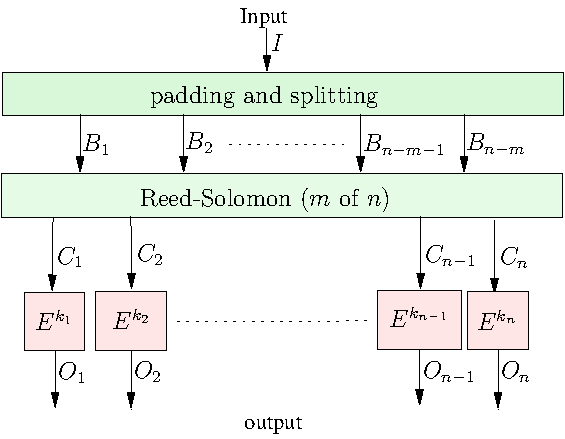
\includegraphics[width=0.8\columnwidth]{inc/addRedundancyOp}
	\caption{Outline of the addRedundancy operation}
	\label{fig:addRedundancyOperation}
\end{figure}

It may be subdivided into the following operations:
\begin{itemize}
	\item Pad the original message block in such a way, that all resulting blocks are a multiple of the block size of the encrypting cipher.
	\item Apply a Reed Solomon operation in a given GF space with a vanderMonde matrix.
	\item Encrypt all resulting blocks with unpadded, symmetrical encryption.
\end{itemize}

%%%%%%%%%%%%%%%%%%%%%%%%%%%%%%%
%%% Preplaced float
%%%%%%%%%%%%%%%%%%%%%%%%%%%%%%%
\begin{figure*}[!t]\centering
	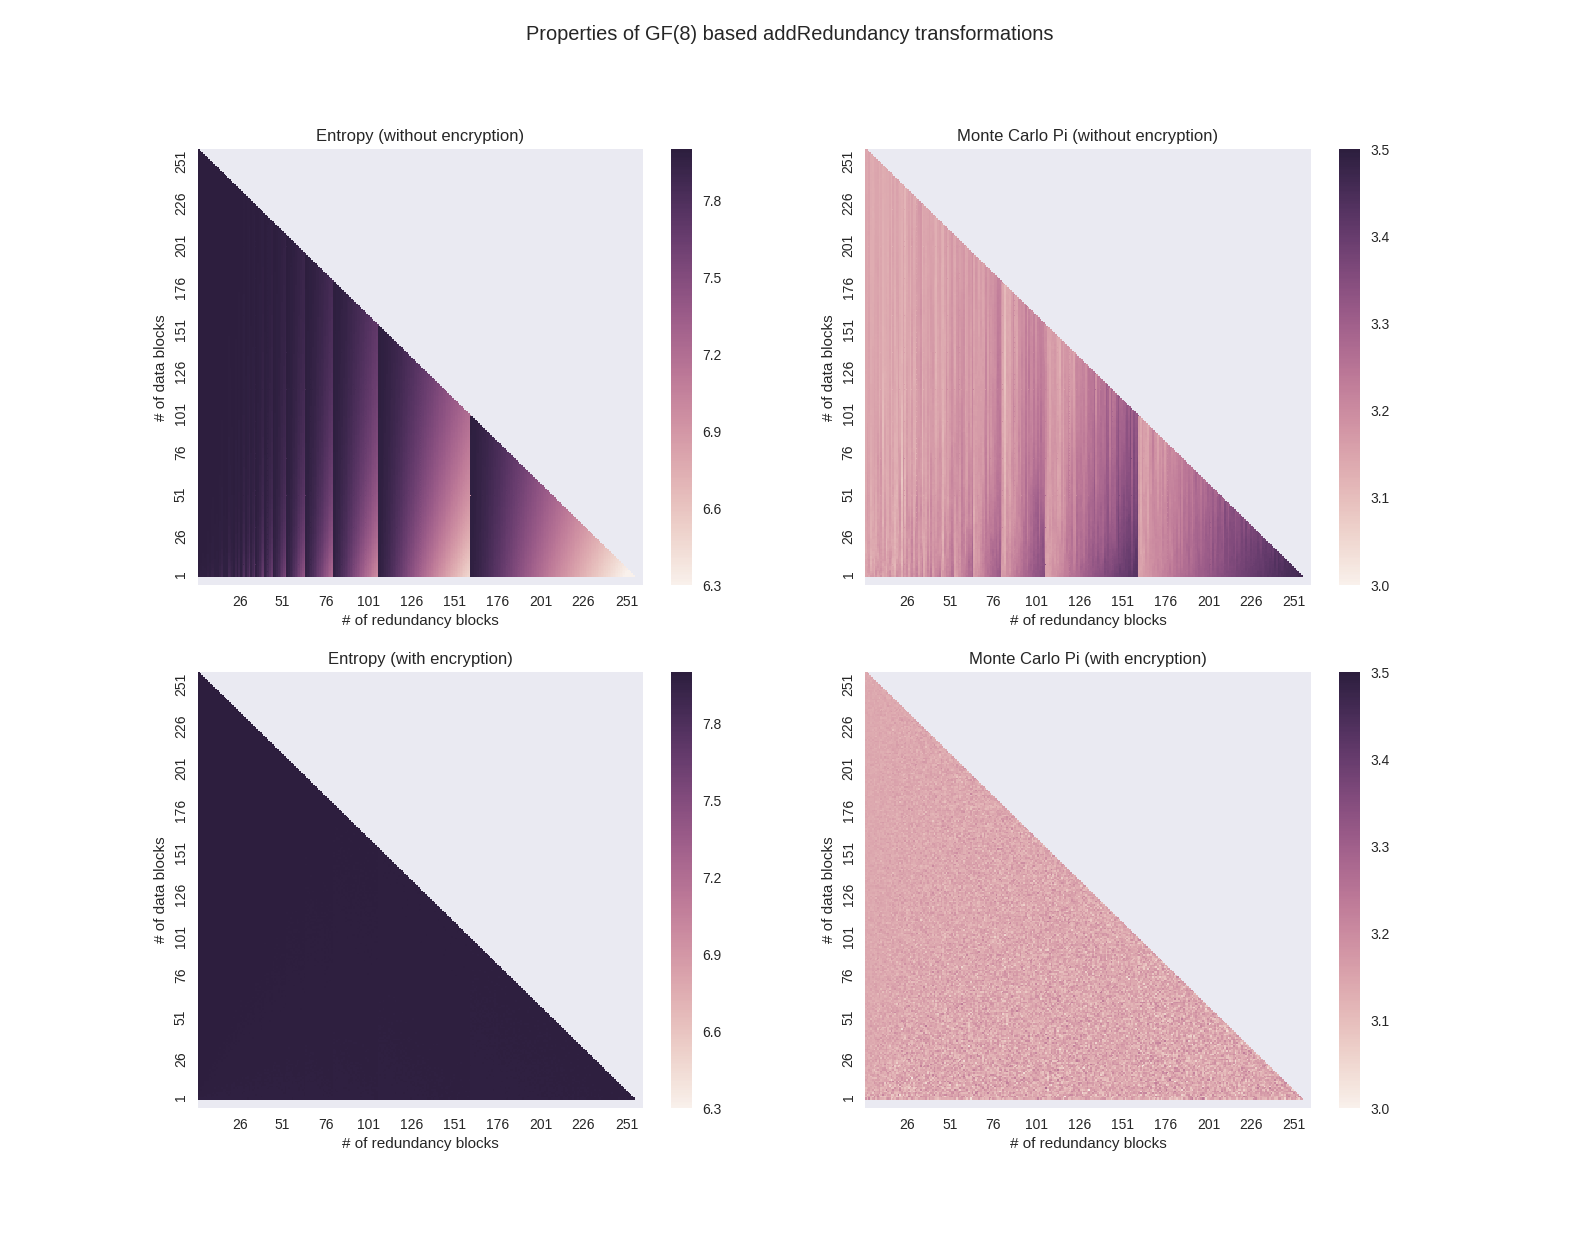
\includegraphics[width=1\textwidth]{inc/randomblock_10kb}
	\caption{Resulting entropy of addRedundancy with and without encryption step}
	\label{fig:entropy}
\end{figure*}



The padding applied in the first step is non-standard padding. The reason for this lies in the properties required by the operation. The presence of standard padding may leak, whether the block has been successfully decrypted or not. Therefore, we created a padding with the following properties:
\begin{itemize}
	\item The padding must not leak whether the rebuild cycle of the operation was successful or not.
	\item Anyone knowing the routing block content and the transmitted message must be able to predict any treated block, including all padding bytes.
	\item The padded content must provide resulting blocks of required size to enable non-padded encryption after the RS operation
	\item The padding must work with any size of padding space.
	\item The padded and encrypted block must not leak an estimate of the original content.
\end{itemize}

The padded block $\mathbf{X}$ is created from a padding value $p$, the unpadded block $\mathbf{M}$ and a series of padding bytes. We build $\mathbf{X}$ for a function $RS_{\text{m of n}}$ and an encryption block $\mathbf{M}$ sized $K$ as follows:
\begin{eqnarray}
i          & = & len(\mathbf{M})\\
e          & = & k \cdot n\\
l          & = & \left\lceil\frac{i + 4 + C2 }{e}\right\rceil\cdot e\\
p          & = & i + \left( C1 \cdot l \pmod{\left\lfloor\frac{2^{32}-i}{l}\right\rfloor\cdot l}\right)\\
\mathbf{X} & = & \langle p,\mathbf{M},R_{t}\left(s,l-i-4\right)\rangle
\end{eqnarray}    
The remainder of the input block, up to length $l$, is padded with random data. The random padding data may be specified by RBB though a PRNG spec $t$ and an initial seed value $s$. The message is padded up to size $L$. All resulting, encrypted blocks do not require any padding. This baecause the initial padding guarantees that all resulting blocks are dividable by the block size of the encrypting function. If not provided by an RBB, an additional parameter $C1$ is chosen as random positive integer and $C2=0$  by the node executing the operation.

To reverse a successful message recovery information the of a padded block $\mathbf{X}$, we calculate the original message size by extracting $p$ and doing $len(\mathbf{M})=p \pmod{ len(\mathbf{X})}$.

This padding has many important advantages:
\begin{enumerate}
	\item The padding does not leak if the rebuilding of the original message was successful. Any value in the padding may reflect a valid value.
	\item Since we have a value $C2$, the statement that a message size is within $len(\mathbf{X})<size<(len(\mathbf{X})-k\cdot n)$ is no longer true and any value smaller $len(\mathbf{X})-k\cdot n$ may be correct as well.
	\item An RBB may predict the exact binary image of the padded message when specifying $C1$, $C2$, and $R_{t}(s,)$.
\end{enumerate}

After the padding, the date is ready for the $addRedundancy$ operation. We first group the data vector into a matrix $\mathbf{A}$ with $m$ columns to do the operations efficiently. The previous padding guarantees that all columns have a length, which is dividable by the block size of the encryption step applied latter.

\begin{eqnarray}
t          & = & n-1\\
\mathbf{A} & = & vec2mat\left(\mathbf{X},\frac{len\left(\mathbf{X}\right)}{m}\right)\\
\mathbf{V} & = & \left(\begin{matrix}
0^0 & 0^1 & 0^2 & \cdots & 0^{(m-1)} \\
1^0 & 1^1 & 1^2 & \cdots & 1^{(m-1)} \\
2^0 & 2^1 & 2^2 & \cdots & 2^{(m-1)} \\
\vdots & \vdots & \vdots & \ddots & \vdots \\
t^0 & t^1 & t^2 & \cdots & t^{(m-1)}
\end{matrix}\right)\\
\mathbf{P} & = & \mathbf{V}\mathbf{A} \left(GF\left(2^\omega\right)\right)\\
\langle \mathbf{Q_1}, \ldots , \mathbf{Q_n} \rangle & = & row2vec(P)\\
R_i & = & E^{K_i}\left(Q_i\right)
\end{eqnarray}    

We do the Reed-Solomon operation by employing a Vandermonde matrix ($\mathbf{V}$). We build the data matrix ($\mathbf{A}$) by distributing the data into $\frac{len\left(\mathbf{X}\right)}{m}$ columns. This results in a matrix with $m$ rows. Unlike in error-correcting systems, we do not normalize the matrix so that the result of the first blocks is equivalent to the original message. Instead, the error-correcting information is distributed over all resulting blocks ($\mathbf{Q_i}$). Since the entropy of the resulting blocks is lowered as shown in figure~\ref{fig:entropy} and may thus leak an estimate of how a resulting block may have been treated, we added the encryption step to equalize entropy again. The previously introduced padding guarantees that there is no further padding on block-level required. The key used to encrypt the single blocks must not be equivalent. Equivalent keys have the side effect encrypting equal blocks into the same cyphertext. We observed faint but statistically relevant reminders of the unencrypted graphs when treating the same block with the same key and different redundancy parameters.

\section{Request Processing}
\emph{VortexMessage} requests allow a Vortex node to gain knowledge about the Vortex network and create new identities. A request may contain either a request for information such as the current quota or capabilities of the router. It may contain a request for a new identity, or it may contain a request for raising the quotas. The following sections explain the different kinds of requests.

\subsection{Requests}
These requests are contained in the header portion of a Vortex message. These requests are purely for bootstrapping and maintaining the quota system and for requesting network capability.

The request information is defined in section \ref{sec:request}. For more information about the exact binary representation of all blocks and data, see chapter \ref{sec:spec}.

Any node decides on its own what type of requests are being answered. 

A node not replying to clear text request is called a ``stealth node'' (see \ref{sec:stealthNode}). Such a stealth node discloses itself only to participants who do already know at least the public key of the node. This usually means that they have ``earned'' this information by issuing a queryPeer request to another node, and obtaining the information did already generate costs to the sender.

A node only replying to a fixed set of identities (in that specific case they are not ephemeral) is called a ``hidden node'' (see section \ref{sec:hiddenNode}).

It is recommended that unencrypted requests are not answered. A node may decide to answer unencrypted queryCapability requests to enable clients to bootstrap without (or with a minimal) network knowledge.

If a message contains $n$ requests in a header block, it must supply at one reply blocks at the beginning of the routing block list. All reply blocks are concatenated and sent using the reply block. If the first block in the routing block list is not a reply block, the request will fail.

\subsubsection{QueryCapability Request}
This request is primarily used to initialize a conversation with a node. It contains valuable information about the capability of the node as well as information about the embedding supported or the encryption. A node may or may not reply to queryCapability requests. Doing so confirms the node to be participating in the vortex network.

The only valid reply is a replyCapability message in encrypted form.

\subsubsection{NewIdentity Request}
If this request is accepted, it generates a new ephemeral identity. The identity itself is stored in the header fields. The standard behavior is to reply with a replyPuzzleRequired block. 

This request generates a temporary, ephemeral identity for the limited time denoted in the validity field of the reply block. No quota is assigned during that phase. As soon as the identity offers a correct puzzle solution, the requested quota is allocated, and the identity may be used for subsequent requests.

If a puzzle is not solved within the given time, the temporary identity may be deleted. A node should not accept a solved puzzle after the given duration. 

Requests with a too high message or transfer quota should not be answered with a replyPuzzleRequired block containing a zero-length puzzle.

\subsubsection{QueryPeer Request}
As outlined in section \ref{sec:request}, this request should be very costly, and the harvesting of public addresses should be hard. Furthermore, this request should always disclose the nodes from a fixed subset of the nodes known to the queried mix. This maximizes the effort to harvest participating nodes.

It is at the same time worth mentioning that this limit may oppose a thread that traffic is concentrated on similar nodes within participating nodes using the same initial set of public addresses to bootstrap. This because if using the same node to bootstrap for multiple participants within a group results in peer knowledge, which is similar. They are thus resulting in a similar network. 

Participants belonging to more than one group will evolve as their different peer partners will result in different anonymity sets over time, even when applying precisely the same reproducible rules.

\subsubsection{TransferQuota, MessageQuota,  and QueryQuota Request}
This request may be accepted by a node if and only if the sender is a valid identity. It may be accepted even for a temporary identity.

The transfer quota offers the capability to raise the number of bytes an identity may transfer. This quota is increased upon request by the ephemeral identity at any time. It is up to the owner of an ephemeral identity and the node using the identity to decide whether an identity may be kept or not, respectively, its quotas raised.

The Message Quota is a quota not limiting the number of bytes but the number of messages. As every message generates accounting overhead, this number has to be limited as well. There are constraints similar to transferQuota when raising this value.

The queryQuota request enables the owner of an ephemeral identity to query the current amount of remaining messages, respectively, bytes.

\subsection{Reply Blocks}
Reply blocks are as outlined in section \ref{sec:replyBlock} prefixed payload blocks. 

\subsubsection{ReplyCapability block}
The replyCapabilityBlock is the reply block to a queryCapability Request. The information provided here is outlined in section \ref{sec:replyBlock}. It is important to note that this block is even when requested in plain is always onionized and thus unreadable for third parties. 

A node may offer different capabilities to known identities than to anonymous clear-text requests.

\subsubsection{replyPuzzleRequired block}


The replyPuzzleRequired block is the block reflecting the payment for a requested operation such as newIdentity, queryPeer, transferQuota, or messageQuota request.

Every puzzle block will create an accounting entry, as outlined in section \ref{sec:accounting}. 

A node may reject an operation for any reason, including exceeding a high amount of outstanding puzzles.

A reply containing a null length puzzle means that the requested operation is rejected.

\section{Protocol Usage\label{sec:spec}}
This approach is different from all approaches discussed previously. Unlike them, we put complete distrust into the infrastructure being used. Furthermore, we do not rely on a custom server infrastructure on the Internet. Instead, we take advantage of the availability of Internet-connected devices such as mobile phones, tablets, or even commonly available SoC such as RaspberryPi or similar. It is still tough to maintain a server on the Internet. Considering the vastly growing amount of automated attacks carried out against Internet-connected servers, it is not advisable or realistic to assume that a future user of this system owns either a server or connects to a service that is offering anonymizing services. These infrastructures would be susceptible to monitoring or even banning. Instead, we take a different approach.

We use common messaging protocols as transport layers and connect to them using the respective client protocols. The actual mixes are operated by the users on their ``always connected'' devices. Such a system is far less reliable than a traditionally run server as this hardware is typically cheap and generally connected to the Internet using a bandwidth shared media.

The basic idea is that a client generates all traffic (including decoy and diagnosis) by itself. It defines the routes a message takes through the mixes and decides which targets are receiving dummy traffic at the same time. In such a system, even when possessing all the nodes routing the traffic (without the endpoints), an anonymity set of $k$ (whereas the sender defines the size of $k$) is guaranteed.

As decoy traffic is generated with the same operations as the real content is split, it is impossible for an adversary running a node to determine whether he is generating noise or processing the real message.
All nodes, regardless of endpoint or mix, implement the same logic, and fulfill the same functions, which make it impossible to determine the function. Exit nodes, as in Tor or similar systems, do not exist.

\section{Accounting}
The Accounting layer maintains all local identities and controls the overall load to the system. He processes requests from an ephemeral identity and generates replies to these requests. 

In table \ref{tab:protoReplyCrit}, we show under what circumstances a reply to a header request should be sent. The capitalized words MAY, MUST, SHOULD, and SHOULD NOT are used as defined in RFC2119\cite{RFC2119}.
\begin{table*}[ht]
	\centering\scriptsize
	\begin{tabular}{|l|l|l|l|l|}\hline
		\diaghead{\theadfont Request Criteria}{Request}{Criteria} & \thead{unknown identity; cleartext} & \thead{unknown identity; encrypted} & \thead{expired identity; encrypted} & \thead{known identity; encrypted}\\\hline
		newIdentity         & SHOULD NOT    & MAY         & Invalid (Error)     & Invalid (Error)\\              
		queryPeer           & MUST NOT      & MUST NOT    & MAY                 & MAY\\        
		queryCapability     & SHOULD NOT    & MAY         & MAY                 & MUST \\
		messageQuota        & MUST NOT      & MUST NOT    & MAY                 & MUST \\              
		transferQuota       & MUST NOT      & MUST NOT    & MAY                 & MUST \\\hline             
	\end{tabular}    
	\caption{Requests and the applicable criteria for replies}
	\label{tab:protoReplyCrit}
\end{table*}

\section{Routing}
The routing of a message is simple. A workspace of an \defref{eID} contains routing blocks and payload blocks. A routing block has an active time window. Anytime during that time window, a routing layer processes the routing instructions contained in the assembly operations of the routing block. If successful, the message will be sent using the specified blending layer and target address.

\section{Blending layer}
The blending layer must be crafted carefully. A blending layer is responsible for the sensible content generation of the transport media plus embedding a \emph{VortexMessage} into the transport layer according to specs provided by the original sender.

The original sender has no control over the plain text messages to avoid the possibility of sending targeted messages over the transport layer using MessageVortex. This differentiates MessageVortex from other systems having ``exit nodes'' such as Tor.

\subsection{Plain Inclusion}
The data stream has of the MessageVortex protocol has no structure visible from the outside. This property allows embedding as structureless information in files with a similar entropy. We did an analysis of common file formats on the Internet to figure out which file format is suitable for this type of inclusion.

It is essential to understand that this is a frail form of information hiding. A human observer may easily tell ``real'' data from ``broken'' data apart. A human is not able to tell whether a file is severely broken or contains a \emph{VortexMessage}.

\subsubsection{File Type Candidates}

We were unable to find any scientifical data regarding what type of traffic or attachment is common on the Internet. We, therefore, tried to analyze mail logs (SMTP) of a mail provider. We were scanning $567594$ emails for attachment properties after the spam elimination queue. $16.5\%$ of all scanned messages had an attachment. The top 20 attachment types distributions are shown in table \ref{tab:emailAttachments}.
\begin{table}[H]
	%    \centering\scriptsize
	
	\begin{tabular}{l|r}\hline
		Type                                                                        & \%\\\hline
		image/jpeg                                                                  &    27.4\\
		application/ms-tnef                                                         &    13.7\\
		image/png                                                                   &    13.3\\
		application/pdf                                                             &    10.7\\
		image/gif                                                                   &    7.4\\
		application/x-pkcs7-signature                                               &    5.4\\
		message/rfc822                                                              &    7.0\\
		application/msword                                                          &    3.1\\
		application/octet-stream                                                    &    3.0\\
		application/pkcs7-signature                                                 &    2.3\\
		application/vnd.\ldots.wordprocessingml.document                            &     1.4\\
		message/disposition-notification                                            &    1.1\\
		application/vnd.ms-excel                                                    &    0.8\\
		application/vnd.\ldots.spreadsheetml.sheet                                  &    0.6\\
		application/zip                                                             &    0.5\\
		application/x-zip-compressed                                                &    0.5\\
		image/pjpeg                                                                 &    0.4\\
		application/pkcs7-mime                                                      &    0.4\\
		video/mp4                                                                   &    0.4\\
		text/calendar                                                               &    0.4\\\hline
	\end{tabular}
	\caption{Distribution of top 20 attachment types}
	\label{tab:emailAttachments}
\end{table}

As expected, the number of images within mail was very high ($\approx 50\%$). Unfortunately, we were unable to analyze the content of ms-tnef attachments retrospectively. It seems that based on these figures, information hiding within images in email traffic is a good choice.

For our implementation, we worked with F5 blending into jpeg images, as this choice seemed to undermine credible content based on table~\ref{tab:emailAttachments}.

\section{Considerations for Building Messages}
In a worst-case scenario, we assume that an adversary is controlling most of the network utilized for anonymization. While this is not necessarily a problem, it allows an adversary to track a message while agents are being used under his control. So for simplicity and as a worst-case assumption, we always assume that an adversary has perfect knowledge of an associated message flow. This is, however, a worst-case scenario. One missing agent disconnects the whole chain, and as messages are no longer traceable.

\subsection{Ephemeral identities}
Any \emph{VortexMessage} sender may maintain one or more ephemeral identities per node. These identities might be active in parallel, overlapping, or even with interruptions. A routing block building node is advised to select multiple trustworthy nodes (such as known endpoints) and add some publicly available nodes or nodes obtained by bootstrapping. Those nodes are not trustworthy and may be chosen from a list of different networks.

\subsection{Timing of messages}
Messages are flowing in a timed manner through the network. As a \defref{RBB} has to take into account that potential routing mechanisms of the transport layer consume time, a message is delayed in each hop.  The \defref{RBB} controls the timing and duration of delivery. Depending on the number of hops for the longest path of the message and the delay windows on every hop, the total message has a delay, which is controllable by the \defref{RBB}.

\subsection{Diagnostics}
To diagnose the flow of a message, any part of the message may be sent directly or indirectly back to the \defref{RBB}. This allows him to judge upon the message progress and whether nodes are well-behaving or not.

There is no fingerprinting operation available for making such a diagnosis. Such operations would make the traffic identifiable as diagnostic traffic.

\subsubsection{Implicit Diagnostic}
When a message contains a routing block sending any parts back to the \defref{RBB}, we call this implicit diagnostic. Any block built by the addRedundancy function may be seen as a kind of fingerprint over the whole message. A block sent back to the originating node may, therefore, reflect the message state up to this point and the way back.

\subsubsection{On-Demand Diagnostic}
Whenever a message fails or suspected fails, a new routing block may be composed picking up parts of the message in workspaces anywhere within the participating nodes. This kind of diagnostic we call On-Demand diagnostic.

On-demand diagnostic allows error conditions identified by implicit diagnostic to be tracked and narrowed down to the first offending node.

\section{Considerations for Routing Messages}
Messages should always be sent nearby other messages timewise. This means that the best moment for sending a message in a ready queue is at a time when sending other messages is due. However, no optimization should be done to send as many messages as possible at the same time. This would lead to a foreseeable behavior of the routing layer and thus to miss-usable behavior.

The approach is furthermore heavily dependent on the transport protocol and builds on top of a new obfuscating/routing layer. For this system to become a real peer-to-peer approach, some additional quirks are required. A message-Vortex-Account always needs an active routing handler. This routing handler may be introduced by new server capabilities or by having a device handling the routing from the client-side. For this reason, we built a RaspberryPi appliance capable of connecting to one (or more) accounts fetching incoming emails, analyzing them, and reroute them if necessary. Although the system is designed to be run on a RaspberryPi, the software might be installed to any Java-capable client. The RaspberryPi is just one affordable, lightweight device that offers all required capabilities.

There was up until very late a routing log functionality in the protocol. This functionality did, however, have the disadvantage that it allowed bugging and could disclose intermediate mixes to a recipient who did not comply with the policy the mixes might have chosen. Therefore this feature was dropped and replaced with the fetch block behavior.

The \defref{RBB} controls the blending. Besides that, he has no control over it. If blending is done carelessly, a message can be easily detected and thus disrupted.

The message leaks its size when a routing block is reused.  This is due to the version number and the ephemeral identity contained in the header. The message chunks reflect approximately the message size compared to the previous message sent.

\chapter{Verification of requirements}
In the previous sections, we identified a list of requirements.

In the following subsections, we will iterate through all requirements and verify to what degree we achieved the goal.

\paragraph*{\ref{req:zeroTrust}:} 
We have not put any trust in an external infrastructure. While we do assume that all routing nodes act as defined. A misbehaving node may be identified and eliminated without putting any trust in other nodes. Analysis has shown no means for a misbehaving node, which might be intentional or unintentional endangering anonymity at any time. We do not rely on any third-party technology or infrastructure for our anonymity. 

This requirement is, therefore, fulfilled.

\paragraph*{\ref{req:P2P}:} 
No node has additional privileges or offers additional services. All are equal and share the same privileges.

This requirement is, therefore, fulfilled.

\paragraph{\ref{req:undetectable}:}
Detectability is highly dependent on the respective implementation of the blending layer. We can clearly state that research in F5 showed no weaknesses so far. Plain blending is not suitable as human censors may detect such blending. 

We did not invest any research effort in the clear text part of the messages. We can clearly state that messages do not have to look like human-generated messages. Status messages from monitoring systems or similar M2H messages are suitable as well. Such messages explain uncommon activities such as 24x7 operation or systematic message outlines. For the academic implementation to be of any value for the public, the current implementation has to be replaced by a blending layer creating suitable content in this respect.

This requirement can be fulfilled, but the current implementation does not meet the required criteria.

\paragraph*{\ref{req:untagable}:} 
Messages may not be tagged. All content is either strictly onionised or defined and linked with unknown hooks. Tampering with a message will typically cause the message delivery to fail at the next node. Furthermore, may tampering be detected.

This requirement is, therefore, fulfilled.

\paragraph*{\ref{req:unbugable}:} 
There are always means to bug a message. As we put trust in the sender and recipient, and we know already that an intermediate mixing node is not able to modify the message, the protocol is hard to bug. There may be a possibility to bug a message with a routing log entry over DNS. If a recipient is not resolving names or trusts in the content of such a message, he is safe.

This requirement is, therefore, fulfilled. It may be only partially fulfilled if log entries are not handled with care.

\paragraph*{\ref{req:replay}:} Messages may only be replayed a limited amount of times. The number of replays is controlled by the sender and may not be altered by any mix. A malfunctioning mix replaying more often than allowed will not be able to extract any information than the information it obtained when sending the first time. 

This requirement is, therefore, fulfilled.

\paragraph*{\ref{req:accounting}:} 
All identities generated are not traceable as any identity is generated without any context and may not be mapped to an older or newer identity (perfect anonymous forward identity). Neither the source nor the replies may be used to be traced as all messages. 

This requirement is, therefore, fulfilled.

\paragraph*{\ref{req:anon}:} Anonymity is hard to proof. 

The following statements are the findings of the previous chapters:
\begin{itemize}
	\item Routing nodes are identifiable by an in-depth inspection.\\
	A routing node features unique features that can be identified. 
	
	Identifyable properties discovered are:
	\begin{itemize}
		\item The usage of the plain embedding is identifiable by a human and using probabilistic approaches even by a scanner.
		\item A router is always connected and sends messages at any time of day
		\item A router is connected to multiple accounts
	\end{itemize}
	\item A routing node can link a message to an ephemeral identity\\
	This is a minor issue and is countered by the fact that ephemeral identities have a very short lifespan and are unconnected.
	\item A routing node learns about other nodes over time.\\
	A routing node is unable to communicate with peers without a host key. It may, however, learn the endpoint address of its peer. Assuming a censoring adversary, this may be a problem in a single case as the provider of the transport layer may be forced to block the account.
\end{itemize}

On the other hand, no node can tell by observing traffic if another node is a final recipient or just another router.

There are, however, some weaknesses in the protocol. As the implementation is currently connecting simultaneously to the transport layer endpoint (email or Jabber account in the current implementation) and the Vortex account, that fact might identify the user. Using an anonymization proxy could solve the problem, but it would violate the Zero trust principle.

A sender is capable of leaking the presence of a receiver to a global observer.

This requirement is, therefore, only partially fulfilled. However, the weakness is very faint.

\paragraph*{\ref{req:boot}:} The header request peer functionality allows to query for routing nodes. The key handling of the protocol allows using a node without disclosing its host key. Each node may decide on whether it leaks its own identity.

This requirement is, therefore, fulfilled.

\paragraph*{\ref{req:algVar}:} The protocol lists at least two completely independent algorithms of each kind to be supported. This allows switching if an algorithm has been broken. Wherever possible, a well-known algorithm and an algorithm basing on an entirely different mathematical problem have been chosen.

This requirement is, therefore, fulfilled.

\paragraph*{\ref{req:easy}:} The protocol allows the use of clients already available and know to the user to send messages. The whole encryption and anonymity problem is hidden in a local proxy. This allows users to stick to their favorite tools.

This requirement is,  therefore, fulfilled.

\chapter{Security Analysis}
In the following sections, we emphasize on attacks targeting either sender-recipient tuples or participating nodes. 

Based on the threat model, we may safely assume the following key points:
\begin{itemize}
	\item An adversary knows and controls a significant number of nodes.
	\item An adversary may observe the traffic at any point without getting any information about the message content
	\item An adversary is not capable of matching multiple messages on different nodes to one message.
\end{itemize}

We always assume an adversary to have more knowledge than we think he may extract from the messages.
\begin{itemize}
	\item We assume that an adversary knows all messages of a transaction running over his nodes and matches them correctly to the same message.
	\item We assume that an adversary is aware of any message only containing decoy traffic.
\end{itemize}

We assume that the adversary is targeting the following pieces of information:
\begin{itemize}
	\item Sender identity
	\item Recipient identity
	\item Message content
	\item Message size
	\item Message frequency
\end{itemize}

Attacks on the users' identity are no longer possible as the identity used on the nodes is based on \defref{eID}s instead of the users' true identity. As the \defref{eID}s may exist in parallel, overlapping, or in a serial manner and are strictly unlinked to the true identity, no statement can be made concerning the linking of ephemeral identities to the real identities. Frequency patterns or behavioral patterns may be split among multiple identities and distributed over multiple nodes. 

Frequency and bandwidth analysis are not possible as the frequency and bandwidth of a single message are not trackable, and the size of a message is generally not related to the message flow. An exception to this statement is when routing a different message through a vortex system using a reused routing block general statements such as ``the message is bigger than the previous one'' about the size of the message is possible if the routing block makes use of relative split operations. In experiments, we were able to mimic any desired communication pattern we wanted for an adversary to be found.

The message content remains cryptographically secured if the dual trust (sender and receiver node) is not broken, the message is encrypted on the senders' node, the message is only decrypted on the node of the receiver, and remains at least wrapped in this encryption during the whole transfer. 

\section{Additional Considerations}

\subsection{Man in the Middle Attacks to Conversations}
Traditional man-in-the-middle (MITM) attacks are not possible when using the \emph{MessageVortex} protocol as the remote identity secures the recipient to a specific recipient. If, however, a recipient identity has been compromised either by stealing its private key or by injecting a wrong identity in the senders' repository man in the middle attacks become possible. We do not cover this problem within this work as a secure, verifiable way to exchange identities is not included in the protocol.

\subsection{Identification of Participating Nodes}
Participating nodes may be identified when injecting evil routing nodes. When suspecting such nodes first step should be moving outside the jurisdictional reach before reaching out to the final anonymity set. If the anonymity set is compromised, identification of the participating nodes is, however, possible.

\subsubsection{Identification by Content}
Message extraction by content is not generally possible even if knowing the blending type and corresponding blending keys. As the \emph{VortexMessage} does not show an outer structure such as ASN.1 or similar. The message itself remains undetectable.

\subsubsection{Identification by Query}
A vortex node may be identified by the query if the node responds to unencrypted requests. An active node may be differentiated from an inactive node at any time if a valid blending specification is known. With such a specification, an evil routing node is capable of creating requests such as new identity requests. As soon as the evil node receives a reply, the node may conclude that the probed node is a VortexNode.

\subsubsection{Identification by Traffic Type}
Vortex node shows a specific behavior in terms of supported protocols. Depending on the implementation, this behavior is detectable. At the moment, supported protocols are POP/SMTP and XMPP. Since both protocols are widespread among Internet users, this footprint is shallow.

\subsection{Storage of Messages and queues}
The storage of messages sent through MessageVortex should be handled with great care. It seems, at first sight, a good idea to merge all messages in globally available storage such as the IMAP account of the receiving entity. However -- In doing so, we would discover the message content to the providing party of a mail account. Since we handled the message with great care and tremendous costs up until this point, it would be careless doing so. 

Storing them in a localized and receiving entity controlled storage is a good idea but leaves security considerations like a backup possibly to an end-user. This might be better but, in effect, a questionable decision. There is, however, a third option: By leaving the message unhandled on the last transport layer of the MessageVortex chain, we may safely back up the data without disclosing the message content. Merging the content then dynamically through a specialized proxy would allow the user to have a unified view on his without compromising the security.

